\documentclass[12pt,a4paper]{report}
\usepackage[utf8]{inputenc}
\usepackage[english]{babel}
\usepackage{amsmath,amsfonts,amssymb}
\usepackage{verbatim}
\usepackage{bm}

\usepackage{tikz}
\usetikzlibrary{shapes,arrows}

\usepackage{hyperref}

\author{Romain Dubessy}
\title{Quantum Simulator -- Reference Manual}

\newcommand{\abs}[1]{\left|#1\right|}
\newcommand{\qsimu}{\texttt{qsimu}\,}
\newcommand{\fft}[1]{\mathcal{F}\left[#1\right]}
\newcommand{\ket}[1]{\left|#1\right>}
\newcommand{\mean}[1]{\left<#1\right>}

\renewcommand{\exp}[1]{\textrm{exp}\left[#1\right]}
\renewcommand{\ln}[1]{\textrm{ln}\left[#1\right]}

\begin{document}
\maketitle
\begin{abstract}
This document is the user's manual of the \qsimu code.
See section~\ref{sec:doc} to generate the programming reference, relative to the source code.
\end{abstract}
\begin{table}
\begin{center}
\begin{tabular}{c|l}
Symbol & Definition \\\hline
$\bm{r}$ & n-dimensional vector\\
$\Delta$ & n-dimensional Laplacian\\
$t$ & Time (in physical units)\\
$m$ & Mass\\
$\hbar=\frac{h}{2\pi}$ & Reduced Planck constant\\
\hline
\end{tabular}
\caption{\label{tab:notations}Some common notation used throughout this document.}
\end{center}
\end{table}
\cleardoublepage
\tableofcontents
\chapter{Introduction}
This program is designed to study the non linear Schrodinger equation (NLSE), also called Gross-Pitaevskii equation (GPE) in the cold atom community:
\begin{equation}
\imath\hbar\frac{\partial}{\partial t}\psi(\bm{r},t)=\left(-\frac{\hbar^2}{2m}\Delta+V(\bm{r},t)+gN\abs{\psi(t,\bm{r})}^2\right)\psi(\bm{r},t),
\label{eqn:gpe}
\end{equation}
white the proper normalisation $\int \bm{dr}\abs{\psi(t,\bm{r})}^2=1$.
Instead of trying to solve Eq.~\eqref{eqn:gpe} with stable algorithms that preserves the wave function normalization, which is not an obvious problem, we will make use of the formal solution of Eq.~\eqref{eqn:gpe} in term of the evolution operator:
\begin{subequations}
\begin{eqnarray}
\psi(\bm{r},t)&=&U(t,t_0)\psi(\bm{r},t_0),\\
U(t,t_0)&=&\exp{-\imath\int_{t_0}^t\frac{dt^\prime}{\hbar}\left(-\frac{\hbar^2}{2m}\Delta+V(\bm{r},t^\prime)+gN\abs{\psi(\bm{r},t^\prime)}^2\right)}.
\label{eqn:evolution}
\end{eqnarray}
\end{subequations}
This is explained with many details in section~\ref{sec:integrator}.

\section{Installation instructions}
First you need to get a working copy of the program.
The code is freely available from a \texttt{git} repository and you can recover the latest stable version with the command:
\begin{verbatim}
$ git clone http://github.com/RDubessy/QSimulator.git
\end{verbatim}
This create a folder \texttt{QSimulator} in your local directory that contains the sources of the program.

The rest of the installation procedure depends on your operating system.

\subsection{Dependencies}
For convenience \qsimu uses dynamically linked external library that provides useful functionalities with optimized code:
\begin{itemize}
\item \texttt{fftw3} a fast Fourier transform library, available at \url{http://www.fftw3.org},
\item \texttt{cvmlib} a \texttt{C++} interface to the famous fortran based linear algebra packages \texttt{blas} and \texttt{lapack}, available at \url{http://www.cvmlib.org},
\item two miscellaneous libraries for the interface with command line options and configuration file, available at \url{http://github.com/RDubessy/MyLibraries},
\end{itemize}
\qsimu assumes that the library files are located in the \texttt{/opt/lib} directory with the corresponding header files in \texttt{/opt/include}.

\subsection{Windows}
Not yet working...

\subsection{Unix/BSD}
In the root directory issue the commands:
\begin{verbatim}
$ make
$ sudo make install
\end{verbatim}
you should now have a working copy of the program in the \texttt{/usr/local/bin} folder.

To test if everything is fine, you can try:
\begin{verbatim}
$ qsimu --usage
\end{verbatim}
which should display some basics about the usage of \qsimu.

\subsection{\label{sec:doc}Getting more documentation}
The code documentation is contained directly in the source files and can be rendered in a more readable way by using the \texttt{Doxygen} tool.
Assuming that \texttt{Doxygen} is installed and properly configured, you can generate the code documentation (as well as the latest version of this reference guide) by issuing:
\begin{verbatim}
$ make doc
\end{verbatim}
in the root directory.
All the related documentation is then placed in the \texttt{doc/} folder, where you will find the reference manual (file \texttt{QSimulator.pdf}) and the code documentation (web pages starting at \texttt{html/index.html}).

\section{Tutorials}
The examples presented here correspond to configuration files in the \texttt{examples/} directory of the program sources.

\subsection{One dimensional harmonic oscillator}
\subsubsection{Defining the problem}
We are interested in the well known harmonic oscillator problem, in one dimension, that can be used as a sandbox to learn how to use \qsimu. 
In this case Eq.~\eqref{eqn:gpe} reduces to:
\begin{equation}
\imath\hbar\frac{\partial}{\partial t}\psi(x,t)=\left(-\frac{\hbar^2}{2m}\frac{\partial^2}{\partial x^2}+\frac{1}{2}m\omega_x^2 x^2\right)\psi(x,t),
\label{eqn:1dho}
\end{equation}
where $\omega_x$ is the trap frequency.

Now we will review, step by step, how to tell \qsimu to solve this problem: first find the ground state, then compute the spectrum of excited states and eventually simulate real time dynamics.

However, for the sake of simplicity, and because it often helps to understand the basic physics, we will now translate \eqref{eqn:1dho} in dimensionless units, using the new variables:
\begin{equation*}
x=a_xX,~t=\frac{T}{\omega_x}~\textrm{and}~\psi(x,t)=\frac{\Psi(X,T)}{\sqrt{a_x}},
\end{equation*}
where $a_x=\sqrt{\frac{\hbar}{m\omega_x}}$ is the characteristic length of the harmonic oscillator.
This results in:
\begin{equation}
\imath\frac{\partial}{\partial T}\Psi(X,T)=\left(-\frac{1}{2}\frac{\partial^2}{\partial x^2}+\frac{1}{2}X^2\right)\Psi(X,T).
\label{eqn:1dlho}
\end{equation}
Now the problem is well posed, and one can see that Eq.~\eqref{eqn:1dlho} has no free parameter: with the dimensional reduction we will be able to obtain results relevant for any (non zero) value of the trapping frequency!

\subsubsection{Writing the configuration file}
The problem has to be defined in a configuration file that \qsimu will use to build a numerical approximation of Eq.~\eqref{eqn:1dho}.
This is done by creating, using your favourite editor, a file \texttt{harmonic1D.cfg} that contains:
\begin{verbatim}
[general]
equation = -1/2*DELTA+VEXT
potential = 1/2*X^2
\end{verbatim}
These three lines tell \qsimu to build a numerical representation of the dimensionless one dimension harmonic oscillator.
Let us see now what is the meaning of these strange lines:
\begin{itemize}
\item\texttt{[general]} is a label that indicates that the next lines will define the problem,
\item\texttt{equation = -1/2*DELTA+VEXT} is the right and side of \eqref{eqn:1dlho},
\item\texttt{potential = 1/2*X\^\,2} is the one dimensional dimensionless harmonic potential.
\end{itemize}

We have now to define a spatial grid on which we will sample the wave function.
This is done by adding a few more lines to our configuration file:
\begin{verbatim}
[grid]
nx = 128
Lx = 30
\end{verbatim}
Again, each line has a particular meaning:
\begin{itemize}
\item \texttt{[grid]} is a label to indicate that the next lines will define the grid,
\item \texttt{nx = 128} is the number of grid points,
\item \texttt{Lx = 30} is the size of the bounding box, in dimensionless units.
\end{itemize}
To be more precise, the grid step size is $dx=\frac{L_x}{n_x}$ and the grid points are: $X_i=-\frac{L_x}{2}+\frac{i}{n_x-1}dx$, so that the grid is symmetric with respect to the center ($X=0$).

The question of choosing the number of grid points and the size of the bounding box is not that trivial an must be considered carefully.
Let us note that the boundary conditions on the borders are not that crucial because, for trapped systems, the density vanishes on the border.
On this particular example we know the analytical solution and therefore we can use it to find a good choice of parameters.
Since it is a sampling problem we will want to have enough grid points not to under sample the distribution but cannot really afford to oversample it, because of memory requirements\footnote{In one dimension this is not really an issue but it will become one in three dimensional problems.}

A good way to tackle this problem will be to consider the rms width of the density distribution: $\sigma_X^2=\int dX\,X^2\abs{\Psi(T,X)}^2$.
In general we will want that the grid satisfies to:
\begin{equation}
dx\ll\sigma_X\ll\frac{L_x}{2},
\end{equation}
such that there is enough points to sample the wave function and that the box is sufficiently large to accommodate it.
Here $\ll$ means that there is an order of magnitude between each of these quantities.
This constraints are certainly necessary but are they sufficient to define an appropriate grid?

The trick is that we work both in real space and in reciprocal space: the grid has to be adapted to the momentum distribution of the wave function.
In the reciprocal space the grid spacing is $dk_x=\frac{1}{L_x}$ while the grid points are defined as: $K_i=-\frac{1}{2dx}+\frac{i}{n}dk_x$.
Let us now define the rms width of the momentum distribution: $\sigma_K^2=\int dK K^2\abs{\fft{\Psi}(K,T)}^2$ and impose the constraints:
\begin{equation}
dk_x\ll\sigma_K\ll\frac{1}{2dx}.
\end{equation}
Let us note that because of Heisenberg uncertainty principle we must have: $\sigma_X\sigma_K\geq\frac{1}{2}$. This impose the a priori constraint to the grid parameters: $dk_x dx\ll\frac{1}{2}$, meaning $n_x\gg2$.

In general the two set of constraints reduce to:
\begin{equation}
L_x\gg2\sigma_X+\frac{1}{\sigma_K}
~\textrm{and}~
n_x\gg\left(\frac{1}{\sigma_X}+2\sigma_K\right)L_x
\label{eqn:gridconstraint}
\end{equation}

In the case of the ground state of Eq.~\eqref{eqn:1dlho}, we know that the inequality is saturated, with $\sigma_X=\sigma_K=\frac{1}{\sqrt{2}}$, and according to the constraints~\eqref{eqn:gridconstraint} it is reasonable to choose $L_x=30$ and $n_x=128$.
Note that it is always better to choose a number of grid points in the form of a power of 2, as fast Fourier transform algorithm are optimized for this case.

\subsubsection{Finding the ground state}
In order to find the ground state of the system we will use the imaginary time propagation algorithm.
To this end we must specify the time step used and the algorithm stopping criteria.
This is done by modifying the configuration file to specify these parameters:
\begin{verbatim}
[general]
equation = -1/2*DELTA+VEXT
potential = 1/2*X^2
dt = 1e-3
tol = 1e-12
dttol = 0.999
[grid]
nx = 128
Lx = 30
\end{verbatim}
where the three new lines stand for:
\begin{itemize}
\item\texttt{dt = 1e-3} the maximum step size used by the algorithm,
\item\texttt{tol = 1e-12} the target relative error on the ground state energy,
\item\texttt{dttol = 0.999} criteria to refine the time step.
\end{itemize}

We are now ready to look for the ground state, hence we run \qsimu with the command line:
\begin{verbatim}
$ qsimu harmonic1D.cfg --groundstate
\end{verbatim}
where the \texttt{--groundstate} option as an obvious meaning.
This command generate a lot of output:
\begin{verbatim}
[I] Initializing problem...
[I] Equation: ((0-((1/2)*DELTA))+VEXT)
[I] Potential: ((1/2)*(X^2))
[I] Getting parameters:
[I] Initializing a 1D Cartesian system
[I] Find groundstate method...
[I]	pass #1 objective: 0.01, done: 3.06735e-05, mu=0.813096
[I]	pass #2 objective: 0.001, done: 3.06735e-05, mu=0.813096
[I]	pass #3 objective: 0.0001, done: 3.06735e-05, mu=0.813096
[I]	pass #4 objective: 1e-05, done: 9.98171e-06, mu=0.501222
[I]	pass #5 objective: 1e-06, done: 9.99144e-07, mu=0.500122
[I]	pass #6 objective: 1e-07, done: 9.9928e-08, mu=0.500012
[I]	pass #7 objective: 1e-08, done: 9.9689e-09, mu=0.500001
[I]	pass #8 objective: 1e-09, done: 9.97424e-10, mu=0.5
[I]	pass #9 objective: 1e-10, done: 9.99201e-11, mu=0.5
[I]	pass #10 objective: 1e-11, done: 9.32587e-12, mu=0.5
[I]	pass #11 objective: 1e-12, done: 2.22045e-13, mu=0.5
[I] After 3372 iterations, mu=0.5 [2.22045e-13].
\end{verbatim}
which we will not comment here but as long as you get lines starting with \texttt{[I]} (information) and not \texttt{[W]} (warning) or even worse \texttt{[E]} (error), everything is fine.

At the end, we see that the algorithm has converged to a value of the energy denoted here \texttt{mu}\footnote{For single particle problems \texttt{mu} stands for the energy while for interacting particles problem it will represent the chemical potential $\mu$.} of $0.49999991666684$, compatible with the expected theoretical value of $\frac{1}{2}$.
Note that the criterion for convergence does not give an accurate estimate of the absolute error on \texttt{mu}: in practice it is difficult to have a relative error below $10^{-7}$.

The printed information is not the only output file: in the current directory a new file has appeared \texttt{psi1.dat} that contains in a binary format the found ground state.

\subsubsection{Plotting the result}
This new file contains the whole state of the system but is not easy to manipulate.
Hopefully, \qsimu can convert it to a more usable form by issuing the command:
\begin{verbatim}
$ qsimu harmonic1D.cfg --in=psi1.dat --plot
\end{verbatim}
This creates two files, located in the \texttt{/tmp/} directory, \texttt{psi\_x.txt} and \texttt{psi\_p.txt}, that contains two representations of the wave function in ascii format: in real and reciprocal spaces.


\subsection{Three dimensional GPE in a harmonic trap}
\subsubsection{Defining the problem}
Let us turn now to the case of a zero temperature degenerate Bose gas confined in a three dimensional harmonic pancake like trap:
\begin{equation}
\imath\frac{\partial}{\partial t}\psi(\bm{r},t)=
\left(-\frac{\hbar^2}{2m}\Delta+\frac{m}{2}(\omega_\perp^2(x^2+y^2)+\omega_z^2z^2)
+gN\abs{\psi(\bm{r},t)}^2\right)\psi(\bm{r},t),
\end{equation}
where $g=\frac{4\pi\hbar^2}{m}a$ is the interaction strength and $N$ the atom number.
Again we will work in dimensionless units using the natural length and energy scale of the vertical harmonic oscillator:
\begin{equation}
\imath\frac{\partial}{\partial T}\Psi(\bm{R},T)=\left(-\frac{\Delta}{2}
+\frac{1}{2}\left(\frac{\omega_\perp^2}{\omega_z^2}(X^2+Y^2)+Z^2\right)
+\frac{4\pi aN}{a_z}\abs{\Psi(\bm{R},T)}^2\right)\Psi(\bm{R},T),
\label{eqn:3dlgpe}
\end{equation}
where $a_z=\sqrt{\frac{\hbar}{m\omega_z}}$, $\bm{r}=a_z\bm{R}$, $T=\omega_zt$ and $\psi(\bm{r},t)=\Psi(\bm{R},T)/a_z^{3/2}$.

Contrary to the previous case, two free parameters remain in equation~\eqref{eqn:3dlgpe}, $\epsilon=\frac{\omega_\perp^2}{\omega_z^2}$ and $g0=\frac{4\pi aN}{a_0}$, for which we have to provide numerical values to \qsimu.
This will be done in the configuration file.

\subsubsection{Writing the configuration file}
We now create a new configuration file \texttt{gpe3D.cfg}:
\begin{verbatim}
[general]
equation = -1/2*DELTA+VEXT+g*RHO
potential = 1/2*(eps*(X^2+Y^2)+Z^2)
dt = 1e-3
tol = 1e-12
dttol = 0.999
[grid]
nx = 32
ny = 32
nz = 32
Lx = 256
Ly = 256
Lz = 16
[parameters]
eps=(25/2000)^2
g=N*eta
N=20000
eta=0.276
\end{verbatim}
The main new features of this file are:
\begin{itemize}
\item the introduction of a new section with the codeword \texttt{[parameters]} that allow to introduce parameters in the \texttt{equation} or the \texttt{potential} definitions.
\item the new term proportional to \texttt{RHO} describing the interactions,
\item a straightforward extension of the previous notations to a three dimensional grid along directions \texttt{X}, \texttt{Y}, \texttt{Z}.
\end{itemize}
The parameter specifications provide great flexibility to the configuration file.
Note however that they must be used with caution: an undefined parameter will cause \qsimu to exit.

Here the chosen numerical values correspond to trap frequencies of $\omega_\perp=2\pi\times25$~Hz and $\omega_z=2\pi\times2000$~Hz and atom number of $20\times10^4$.

\subsubsection{Studying the ground state}

\chapter{Configuration file}
Note that the configuration file is parsed line after line, so that expressions should be defined on a single line. Empty spaces or tabulations are discarded, as well as everything following the symbol \texttt{\#} that can be used to write comments in the file.

\section{\label{sec:codewords}Codewords}
Hereafter is the list of all the configuration file reserved words that have a special meaning for the program.
User defined parameters should bear other names.
For convenience the following list is alphabetically sorted.
\begin{itemize}
\item \texttt{DELTA} represents the Laplacian in the \texttt{equation}. It is implicitly defined by the choice of coordinate system in the \texttt{potential} assignation.
\item \texttt{equation = ...} represents the integrand of the evolution operator defined in equation~\eqref{eqn:evolution}. It should be written in the form:\\ \texttt{equation = A*DELTA+B*VEXT+C*RHO+D*LZ}, where \texttt{A}, \texttt{B}, \texttt{C} and \texttt{D} are user defined parameters.
\item \texttt{[general]} is label indicating the general configuration options.
\item \texttt{[grid]} is a label indicating the beginning of the spatial grid definition.
\item \texttt{LZ} represents the projection along the z axis of the angular momentum operator. It can be used to simulate a rotating frame. 
\item \texttt{[parameters]} is a label indicating the beginning of the user defined parameters assignation.
\item \texttt{potential = ...} defines the spatial dependence of the trapping potential. It can use either Cartesian coordinates (\texttt{X}, \texttt{Y} and \texttt{Z}) or cylindrical coordinates (\texttt{R}, \texttt{THETA}, \texttt{Z}), that may by combined using mathematical expressions.
\item \texttt{RHO} represents an interaction term proportional to the local particle density.
\item \texttt{VEXT} represents the external trapping potential in the \texttt{equation}. Its value is defined in the \texttt{potential} assignation.
\end{itemize}

\section{Mathematical expressions}
It is possible to use arbitrary mathematical expressions in the configuration file.
These are parsed using an external library capable of recognizing: elementary operations, variables and simple mathematical functions, according to a specific syntax.
Mathematical expressions may be grouped or delimited by matching pairs of parenthesis \texttt{(...)} that may be nested to an arbitrary level.

\subsection{Elementary operation}
The elementary operation currently supported are:
\begin{itemize}
\item \texttt{+} addition,
\item \texttt{-} subtraction,
\item \texttt{*} multiplication,
\item \texttt{/} division,
\item \texttt{\^} power.
\end{itemize}
Note that the usual algebra rules apply (distributive, associative and commutative properties).

\subsection{Mathematical functions}
Mathematical functions are written as \texttt{Name[...]} where \texttt{Name} is a short name for the function and the argument is written between square brackets \texttt{[...]}.
The functions implementation rely on the standard mathematical library of your operating system.

The mathematical functions currently supported are:
\begin{itemize}
\item \texttt{Exp[...]} the exponential function,
\item \texttt{Sqrt[...]} the square root function,
\item \texttt{Erf[...]} the error function,
\item \texttt{Cos[...]} the cosine function,
\item \texttt{Sin[...]} the sine function,
\item \texttt{Tan[...]} the tangent function,
\item \texttt{Cosh[...]} the hyperbolic cosine function,
\item \texttt{Sinh[...]} the hyperbolic sine function,
\item \texttt{Tanh[...]} the hyperbolic tangent function.
\end{itemize}

\section{Coordinate systems and grid definition}
The coordinate system used for the computation is implicitly defined by the expression of the trapping potential.
This potential may be expressed either in Cartesian coordinates (\texttt{X}, \texttt{Y} and \texttt{Z}) or cylindrical coordinates (\texttt{R}, \texttt{THETA}, \texttt{Z}).
The choice of the coordinate system defines the Laplacian \texttt{DELTA}.
The current implementation of the program allows for:
\begin{itemize}
\item \texttt{X}: one dimensional problem with $\Delta=\frac{\partial^2}{\partial x^2}$,
\item \texttt{X}, \texttt{Y}: two dimensional problem with $\Delta=\frac{\partial^2}{\partial x^2}+\frac{\partial^2}{\partial y^2}$,
\item \texttt{X}, \texttt{Y}, \texttt{Z}: three dimensional problem with $\Delta=\frac{\partial^2}{\partial x^2}+\frac{\partial^2}{\partial y^2}+\frac{\partial^2}{\partial z^2}$,
\item \texttt{R}: one dimensional polar problem with $\Delta=\frac{\partial^2}{\partial r^2}+\frac{1}{r}\frac{\partial}{\partial r}$.
\end{itemize}


\chapter{Numerical methods}
\section{\label{sec:integrator}Split operator and fast Fourier transforms}
The basic idea is to approximate the small step evolution operator $\delta U(t)=U(t+dt,t)$ by using a Trotter expansion:
\begin{eqnarray*}
\delta U(t)
&=&\exp{-\imath\frac{dt}{\hbar}\left(-\frac{\hbar^2}{2m}\Delta
+V(\bm{r},t)+gN\abs{\psi(\bm{r},t)}^2\right)}\\
&\simeq&\exp{\imath\frac{dt}{\hbar}\frac{\hbar^2}{2m}\Delta}
\times
\exp{-\imath\frac{dt}{\hbar}\left(V(\bm{r},t)+gN\abs{\psi(\bm{r},t)}^2\right)}
+\mathcal{O}\left(dt^2\right)\\
%&+&\frac{dt^2}{2\hbar^2}\left(\left(V(\bm{r},t)+gN\abs{\psi(\bm{r},t)}^2\right)\frac{\hbar^2}{2m}\Delta-\frac{\hbar^2}{2m}\Delta\left(V(\bm{r},t)+gN\abs{\psi(\bm{r},t)}^2\right)\right)
\end{eqnarray*}
This formulation allows to keep a unitary evolution, with two successive steps, easy to evaluate respectively in the real and reciprocal spaces, at the cost of a small error of order $dt^2$.
This error may be evaluated globally as:
\begin{eqnarray*}
\epsilon&=&-\frac{dt^2}{4m}\mean{\left[\Delta,V(\bm{r},t)+gN\abs{\psi(\bm{r},t)}^2\right]}.
\end{eqnarray*}

\section{Imaginary time propagation}
\begin{figure}[htbp]
\begin{center}
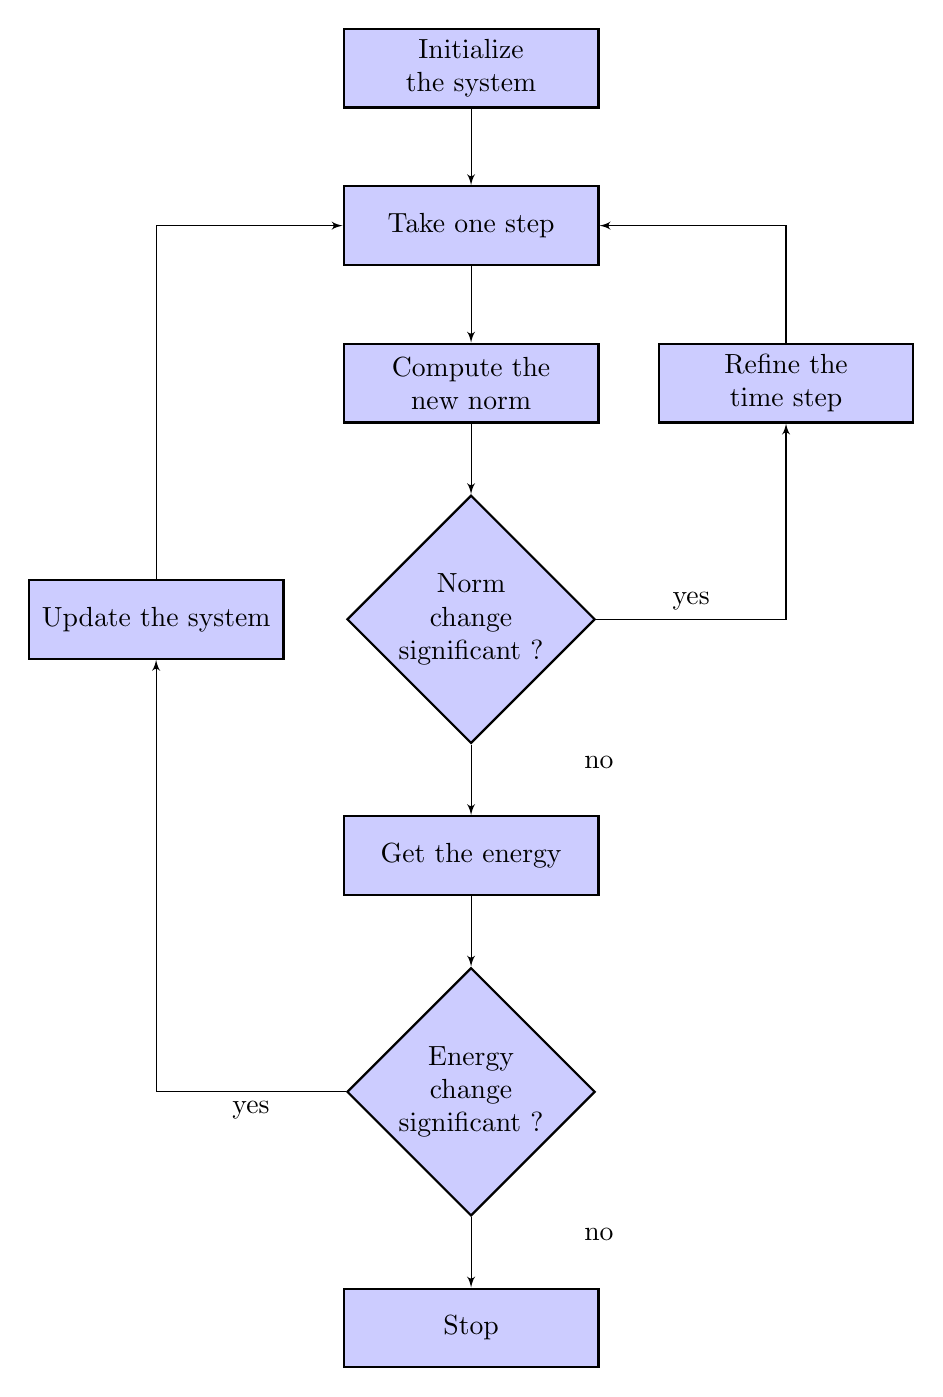
\begin{tikzpicture}[auto,text width=3cm,node distance=2cm,text centered,
	block/.style={rectangle,draw=black,fill=blue!20,thick,minimum height=1cm},
	test/.style={diamond,draw=black,fill=blue!20,thick,inner sep=0pt,text width=2cm},
	line/.style={draw,-latex'}]
\node[block] (input) {Initialize the system};
\node[below of=input,block] (step) {Take one step};
\node[below of=step,block] (normalize) {Compute the new norm};
\node[right of=normalize,block,node distance=4cm] (refine) {Refine the time step};
\node[below of=normalize,test,node distance=3cm] (test) {Norm change significant ?};
\node[left of=test,block,node distance=4cm] (update) {Update the system};
\node[below of=test,block,node distance=3cm] (energy) {Get the energy};
\node[below of=energy,test,node distance=3cm] (test2) {Energy change significant ?};
\node[below of=test2,block,node distance=3cm] (output) {Stop};
\path[line] (input) -- (step);
\path[line] (step) -- (normalize);
\path[line] (normalize) -- (test);
\path[line] (test) --node[near start] {no} (energy);
\path[line] (test) -|node[near start] {yes} (refine);
\path[line] (refine) |- (step);
\path[line] (energy) -- (test2);
\path[line] (test2) --node[near start] {no} (output);
\path[line] (test2) -|node[near start] {yes} (update);
\path[line] (update) |- (step);
\end{tikzpicture}
\caption{Chart flow of the imaginary time propagation algorithm. Detail of one pass.}
\end{center}
\end{figure}

\section{Spectrum of excitations}
Assuming that $\psi_0(\bm{r})e^{-\imath\frac{\mu}{\hbar}t}$ is a stationary state of equation~\eqref{eqn:gpe}, with a time independant potential $V(\bm{r},t)=V(\bm{r})$, one can look for elementary excitations around this state in the form: $\psi(\bm{r},t)=e^{-\imath\frac{\mu}{\hbar}t}
\left(\psi_0(\bm{r})+\delta\psi(\bm{r},t)\right)$.
Assuming $\abs{\delta\psi(\bm{r},t)}\ll\abs{\psi_0(\bm{r})}$ and linearising equation~\eqref{eqn:gpe}, one get the following first order equation:
\begin{equation}
\imath\hbar\frac{\partial}{\partial t}\delta\psi(\bm{r},t)
=\mathcal{L}\delta\psi(\bm{r},t)+gN\psi_0(\bm{r})^2\delta\psi(\bm{r},t)^*,
\label{eqn:gpelin}
\end{equation}
where we introduced the operator:
$\mathcal{L}=\left(-\frac{\hbar^2}{2m}\Delta+V(\bm{r})+2gN\abs{\psi_0(\bm{r})}^2-\mu\right)$.
This equation is not linear in $\delta\psi(\bm{r},t)$ because of the term $\delta\psi(\bm{r},t)^*$ but can be transformed to a set of linear equations by using the Bogoliubov transformation:
\begin{equation}
\delta\psi(\bm{r},t)=\sum_k\left(u_k(\bm{r})e^{-\imath\omega_kt}
+v_k(\bm{r})^*e^{\imath\omega_k^*t}\right),
\label{eqn:bogo}
\end{equation}
where $k$ is a label identifying the modes.
Plugging the transformation~\eqref{eqn:bogo} into equation~\eqref{eqn:gpelin} one gets:
\begin{subequations}
\begin{eqnarray}
\hbar\omega_ku_k(\bm{r})&=&\mathcal{L}u_k(\bm{r})+gN\phi_0(\bm{r})^2v_k(\bm{r}),\\
-\hbar\omega_kv_k(\bm{r})&=&\mathcal{L}^*v_k(\bm{r})+gN\phi_0(\bm{r})^{*2}u_k(\bm{r}).
\end{eqnarray}
\end{subequations}
This system is now linear and we must find the eigenvalues and eigenvectors of the operator: $\begin{pmatrix}
\mathcal{L} & gN\abs{\psi_0(\bm{r})}^2\\
-gN\abs{\psi_0(\bm{r})}^{*2} & -\mathcal{L}^*
\end{pmatrix}$.
It can be shown that the proper normalization for the eigenvectors is:
\begin{equation}
\int d\bm{r}\left(\abs{u_k(\bm{r})}^2-\abs{v_k(\bm{r})}^2\right)=1.
\end{equation}

\appendix
\chapter{Getting more by using scripts}
It is possible to override the configuration files values by assigning the parameters values directly from the command line interface.
Indeed \qsimu accepts options of the form: \texttt{--label::symbol=...} where \texttt{label} is one of the label codewords of the configuration file and \texttt{symbol} is one of the parameters related to this codeword (see section~\ref{sec:codewords} for details).
For example, it is possible to specify the number of grid points this way:
\begin{verbatim}
$ qsimu harmonic1D.cfg --grid::nx=128 --groundstate
\end{verbatim}
Note that \qsimu accepts options in any order.

This possibility makes easier the creation of short scripts to study the same problem with small variations.

\chapter{Finite temperature}
System ground state in dimension $d$:
\begin{subequations}
\begin{eqnarray}
\mu \phi_0(\bm{r})&=&\left(-\frac{\hbar^2}{2m}\Delta+V(\bm{r})+g\left(\abs{\phi_0(\bm{r})}^2+2n_0(\bm{r})\right)\right)\phi_0(\bm{r})\\
n_0(\bm{r})&=&\int\frac{d^d\bm{p}}{h^d}
\frac{1}{z(\bm{r})^{-1}\exp{\beta\frac{\bm{p}^2}{2m}}-1}
=\frac{1}{\Lambda^d}g_{d/2}\left(z(\bm{r})\right)
\end{eqnarray}
\end{subequations}
where: $z(\bm{r})=\exp{-\beta\left(V(\bm{r})+2g\left(\abs{\phi_0(\bm{r})}^2+n_0(\bm{r})\right)-\mu\right)}$ is the local equilibrium fugacity, $\Lambda=\sqrt{\frac{h^2\beta}{2\pi m}}$ is the thermal de Broglie wavelength and $g_s(z)=\sum_{n=1}^\infty\frac{z^n}{n^s}$ is the Polylogarithm function.

Note that for dimension $d=2$ the Polylogarithm has the analytical form: $g_1(z)=-\ln{1-z}$.
\end{document}